\documentclass{lug}

\title{OpenGL \& Computer Graphics}
\author{Sam Sartor}
\institute{Mines Linux Users Group}

\usepackage{etoolbox}
\usepackage{array}
\usepackage{amsmath}
\usepackage{adjustbox}

\makeatletter
\patchcmd{\beamer@sectionintoc}{\vskip1.5em}{\vskip0.5em}{}{}
\makeatother

\begin{document}

\newcommand{\teapotrtpix}{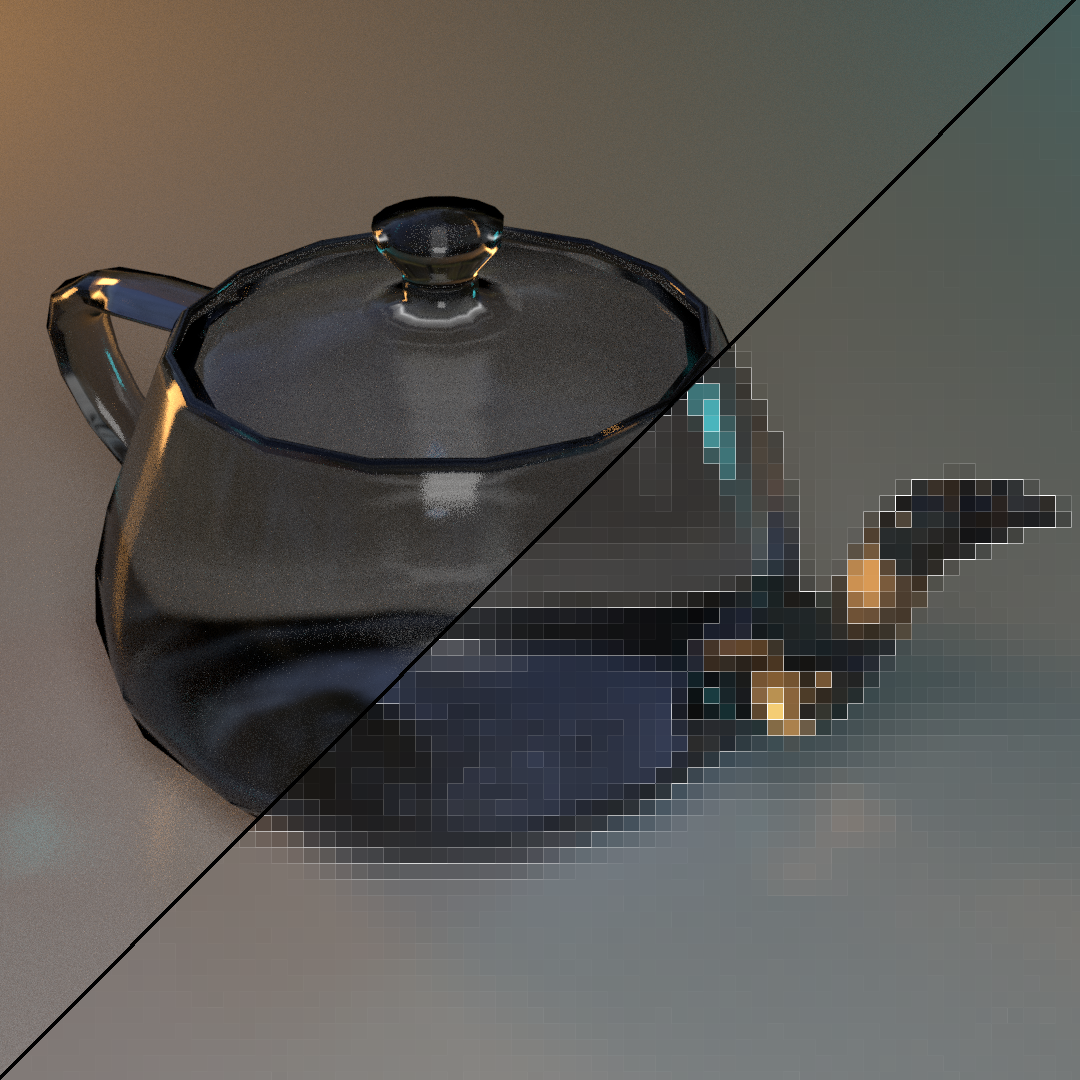
\includegraphics[width=4cm]{graphics/teapot_rt_pix}}
\newcommand{\teapotmesh}{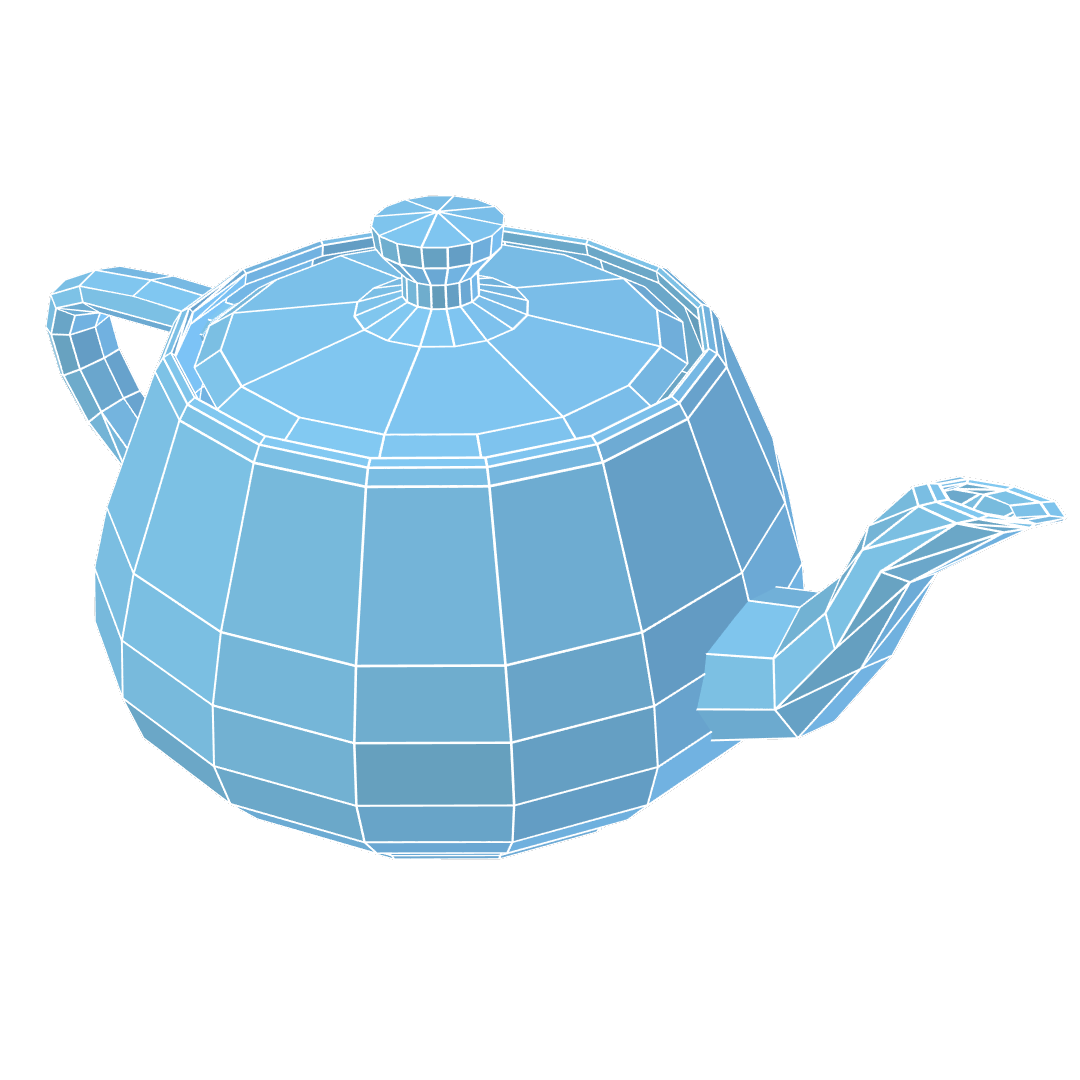
\includegraphics[width=4cm]{graphics/teapot_mesh}}

\begin{frame}{What is Computer Graphics}
\begin{center}
    \parbox{\widthof{\teapotmesh}}{\teapotmesh} \scalebox{2}{$\rightarrow$} \parbox{\widthof{\teapotrtpix}}{\teapotrtpix} \\
    
    \bigskip

    Computer graphics is the science of turning \textit{shapes} into \textit{pixels}.
\end{center}
\end{frame}

\begin{frame}{Offline vs Online}
\end{frame}

\begin{frame}{History}
\end{frame}

\end{document}
